\section{Serialization overheads}

At the end of the day, any consistent memory model requires some form
of serialization.  Indeed, it is well known that sequential
consistency can be implemented by ensuring that all operations on a
given memory address are totally ordered~\cite{ivy}.  In this section,
we survey the alternatives available in existing RDMA hardware, ranging from optimistic approaches that detect and recover from reordering to those that enforce varying degrees of serialization.

\subsection{RDMA costs}

In principle, clients can deal with potential conflicts by utilizing the atomic
operations provided by the RDMA specification, such as compare and swap (CAS).
Like their local CPU counterparts, CAS enables (seemingly) lock-free updates to
far data by detecting races and allowing clients to implement recovery
mechanisms. In practice, however, these atomics are
famously~\cite{design-guidelines,clover} expensive, fundamentally because they
require mutual exclusion across all queue pairs to deliver their functionality.
As shown in prior work~\cite{design-guidelines}[Figure. 14], the rate at which
atomics bottleneck is a function of their addresses being independent from one
another.

The execution of CAS on a NIC is further slowed by it's distance from the memory
on which it's transaction is performed. The NIC determines the address to lock,
ensures that no dependent writes are concurrent, then performs the write, and
waits for the PCIe transaction to main memory to complete. The PCIe bus adds
latency to the operation. This separation between the decision making point
(NIC) and the location of execution (main memory) causes another fundamental
overhead in using RDMA based atomics. Ideally the decision point and execution
of location would have minimal latency. i.e CPU and L1 cache.

\begin{figure}[t]
    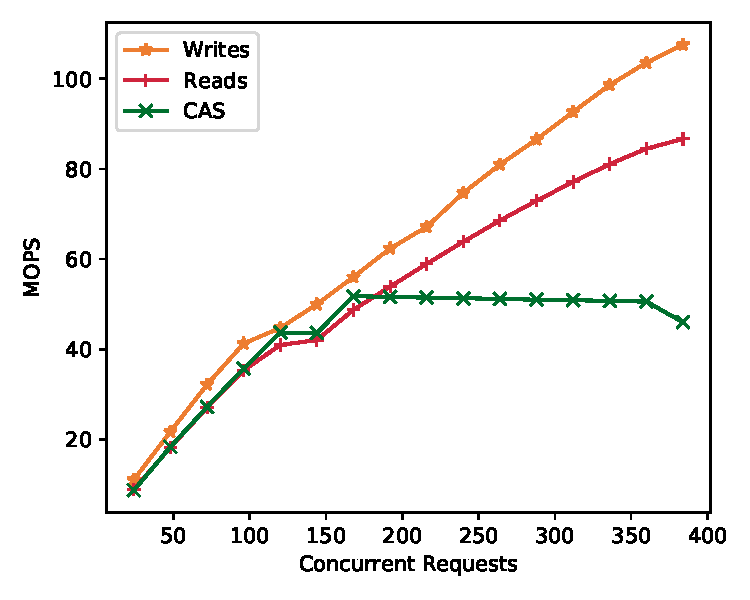
\includegraphics[width=0.45\textwidth]{fig/rdma_concur.pdf}
    \caption{Relative Speed of RDMA verbs as a function of parallel requests}
    \label{fig:rdma_concur}
\end{figure}

RDMA is designed for extremely high throughput and low latency operations. Far
memory systems use their verb library to implement remote memory operations. The
most common are reads, and writes, with the atomic library being used to
implement serialized remote memory accesses. Atomics operations require
significantly NIC memory and are substantially slower than default reads and
writes. Figure~\ref{fig:rdma_concur} Is a benchmark of RDMA verb performance
between two ConnectX-5 NICs. Note that read and write performance are able to
achieve approximately 2x the performance of the atomic CAS instruction.

RDMA atomic operations are known to be slow due to their need to make a PCIe
round trip. In contrast locks held in SRAM require only a few nanoseconds to
perform locking operations. To unlock the full potential of RDMA we convert
compare and swap operations to writes in network. While this operation is
generally unsafe, by resolving all conflicts, and using RDMA reliable
connections, we can ensure all operations succeed and serialization without
using RDMA atomic operations.

\subsubsection{Read tearing}
\todo{place somewhere else}
Async reads and writes can lead to read tearing. Reads
will happily occur on address which are mid write. Writes are done per cache
line, but can span many. To prevent corruption writes are typically followed by
a checksum which provides data integrity~\cite{pilaf,clover}. One advantage of CAS is
that it ensure all reads are complete even if the 64 byte CAS is across cache
lines.

\subsubsection{Memory management hardware}

Hence, a performant far memory system should avoid the use of atomic operations
if at all possible, relying instead on async RDMA verbs.  Even in that case,
existing hardware does provide some guarantees.  For example, RDMA provides
access to memory hosted on a server that likely utilizes a commodity hardware
memory management unit (MMU).  All modern MMUs ensure coherent memory accesses,
and generally ensure a total ordering on local memory requests.  Unfortunately,
due to the complexities of today's multi-core NUMA architectures and PCIe bus
arbitration, it is possible that memory requests may not be serviced in the
order they are dispatched. Happily, the RDMA specification requires that NICs
enforce ordering across operations in an individual queue pair, so sequential
consistency can be ensured by ensuring that all requests for a given memory
location arrive on the same queue pair.


\todo{modify this paragraph so that it is closer to the truth}
Figure~\ref{fig:reorder} shows that this guarantee is actually required: i.e.,
requests across queue pairs are \emph{not} always processed in the order
received in practice.  In this example, we use RDMA \texttt{t\&s} operations to
detect reordering.  Specifically, we generate a sequence of test-and-set
operations that increment the value stored at the indicated location by one if
and only if the current value is as expected, i.e., one lower.  Because we
ensure the operations are delivered to the NIC sequentially, a failed operation
indicates the request was reordered internal to the remote server.  We generate
operations for 1,000 different physical addresses (according to a Zipf
distribution) using a varying number of queue pairs and report the frequency
with which they are reordered with respect to another request for the same
address (i.e., the \texttt{t\&s} operation fails).  As expected, when all
requests are issued on the same queue pair, they are serviced in order.  Once a
non-trivial level of concurrency is reached, however, the reordering becomes
significant, with over 7\% of requests to the same address serviced out of order
when they are spread across 32 queue pairs.\sg{given a zipf distribution, and
16qp around 3\% of packets are reordered. This is detected by checking the
sequence numbers against the known monotonic sequence.}

\begin{figure}[t]
    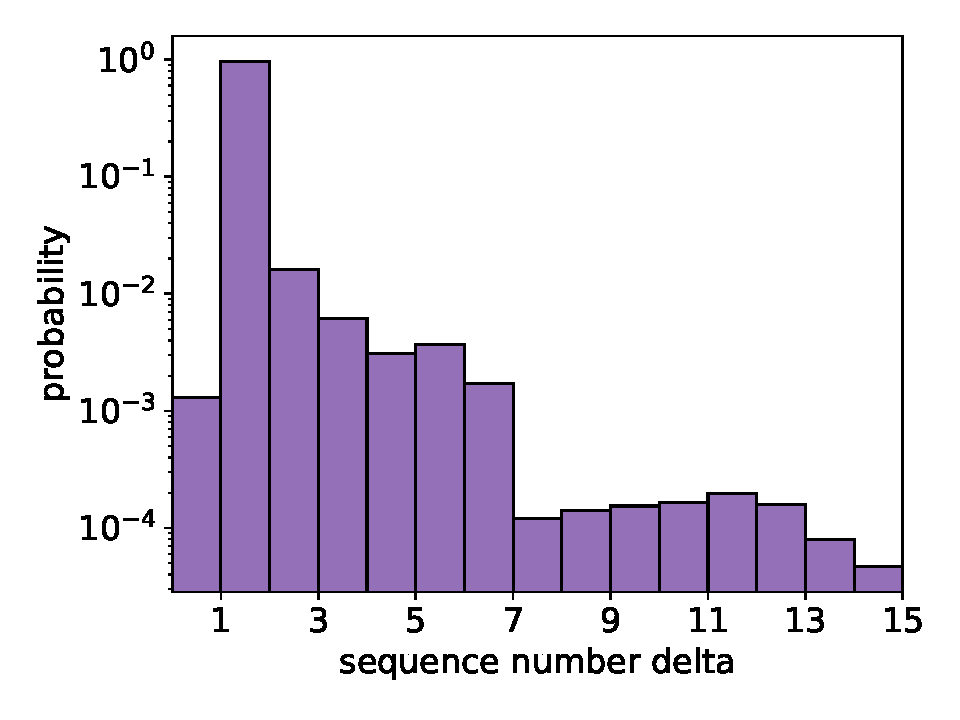
\includegraphics[width=0.45\textwidth]{fig/qp_reordering.pdf}
    \caption{CDF of packet reorderings once QP mapping is applied to a zipf distribution}
    \label{fig:reorder}
\end{figure}

\subsubsection{Queue pair bottlenecks}

 There are two challenges to restricting requests for a given address
 to a single queue pair---one that can be worked around, and one that
 must be addressed.  First, queue pairs are established on a
 client/server basis, so requests from different clients must arrive
 on different queue pairs.  Second, the performance of a single queue
 pair on commercial NICs is significantly less than line rate (likely
 precisely because of the need to enforce ordering constraints).

\begin{figure}[t]
    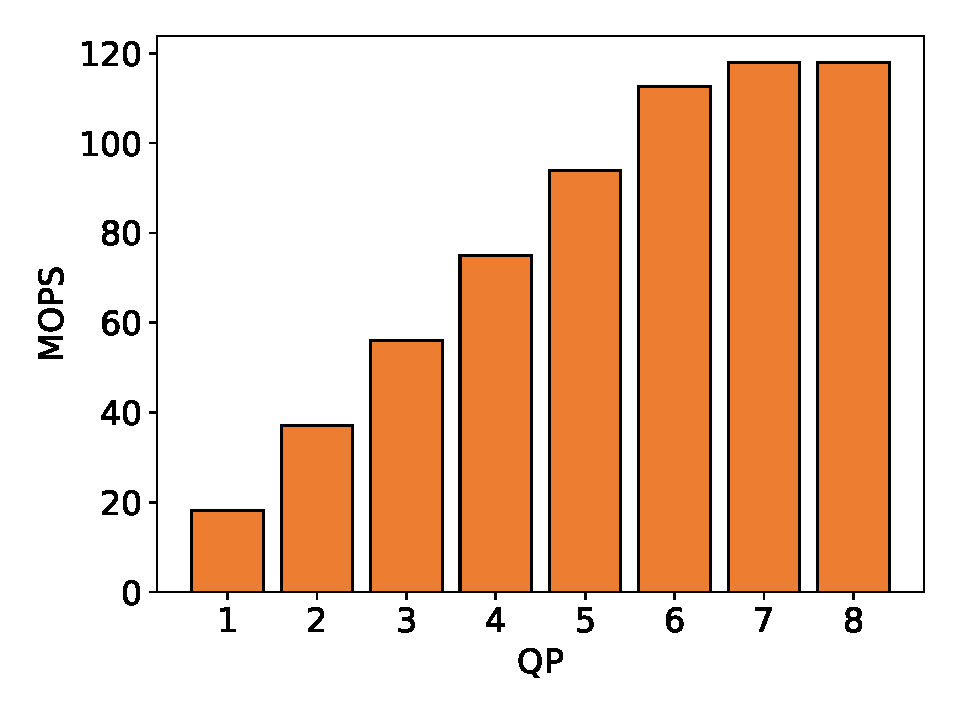
\includegraphics[width=0.45\textwidth]{fig/qp_bottleneck.pdf}
    \caption{Max throughput per QP \todo{take real measurement}}
    \label{fig:qp_bottleneck}
\end{figure}



\subsection{Conflict resolution}

Sharing remote memory creates a variety of performance problems related to
synchronization. Some problems are system, and algorithm specific, while others
are the result of RDMA hardware limitations. 

If synchronization techniques such as spinlocks were naively
implemented the cost of acquiring the lock would be multiplied by many orders of
magnitude. As such developers of remote memory systems typically rely on
optimistic concurrency mechanisms so that in cases were no contention exists
remote operations can succeed on their first try.

\begin{figure}[t]
    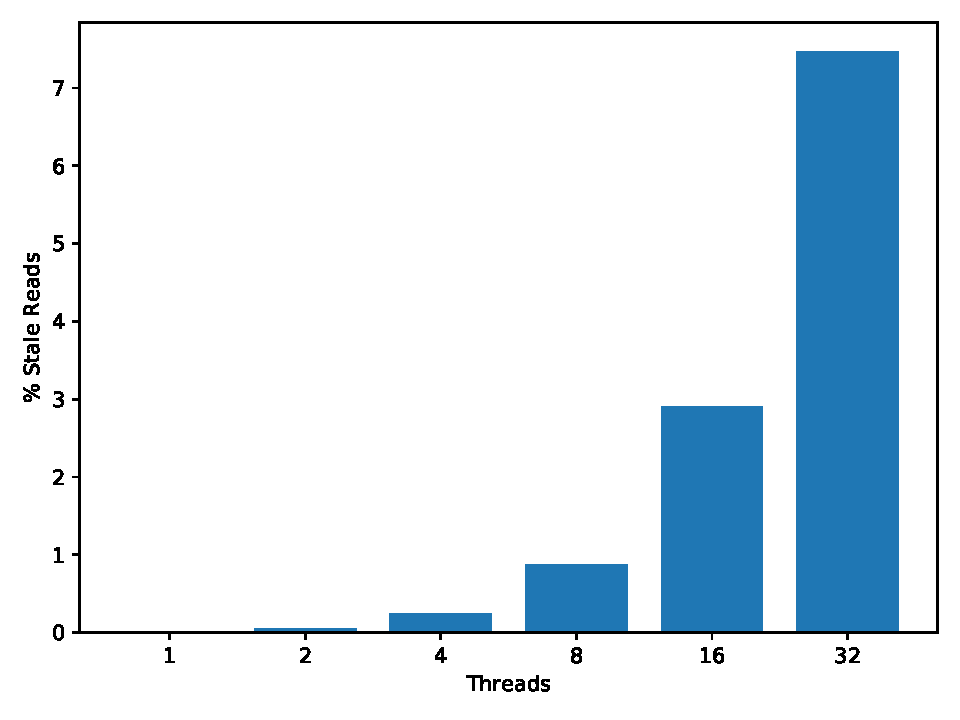
\includegraphics[width=0.45\textwidth]{fig/stale_reads.pdf}
    \caption{Percentage of stale reads made on a 50\% write workload}
    \label{fig:stale_reads}
\end{figure}

Optimistic concurrency algorithms are by definition optimistic, and when
contention does occur their operations must be retried in order to complete the
operation. Clover's opportunistic algorithm attempts to read and write to the
tail of a list for each key, in it's key value store. The location of the tail
of the list is guessed opportunistically (it moves on every write). If the guess
is incorrect the algorithm retries. Both writes and reads can fail, and must be
retried. Figure~\ref{fig:stale_reads} shows the percentage of reads which fail
at a 50\% write workload in clover \footnote{Write fail at a nearly identical
rate}. Retried operations result in large throughput drops (2x) and massive
increases in tail latency (26x) We correct for these opportunistic failures by
caching the location of the most recent writes, and using them to steer
operations from old locations to the most up to date. Ensuring that operations
do not fail drastically improves overall performance under contention. However
some performance is still left untapped as the underlying RDMA hardware has
further limitations. 

\subsubsection{Bandwidth Inflation} 

Optimistic concurrency is designed to have low cost common case operations and
only incur a penalty when conflicts occur. The typical strategy to deal with
conflicts is to arbitrarily determine a winner, and have the loser retry. With
remote memory retires consume network bandwidth and resources. As contention
increases so to does the average cost of each operation. Our results show that
under contention the average cost of read and write operations can inflate by up
to 2x Figure~\ref{fig:bandwidth_reduction} above an optimal O(1) implementation when
all operations succeed on their first try.

\subsubsection{Tail Latency}

High tail latencies are a well understood bottleneck which greatly effect
end-to-end system performance. Under contention optimistic concurrency
mechanisms can exhibit extreme tail latencies. Our experimentation with Clover
shows that under moderate write pressure (50\% write operations with 64 threads)
it's 99th tail latency increases by 83x Figure~\ref{fig:tail_latency}. Reducing the
cost of each operation to exactly 1 attempt can reduce this additional latency
by nearly two orders of magnitude.








